\documentclass[a4paper,10pt,oneside]{article}
\usepackage[polutonikogreek,italian]{babel}
\usepackage[utf8x]{inputenc}
\usepackage{amsmath}
\usepackage{amsthm}
\usepackage{amssymb}
\usepackage{amscd}
\usepackage{graphicx}
\usepackage{float}
\usepackage{array}
\usepackage{rotating}
\usepackage[small]{caption}
\usepackage{lscape}
\usepackage{fancybox}
\usepackage{booktabs}
\usepackage[noanswer]{exercise}
\usepackage{wasysym}

\def\Arrow{\raisebox{-.5\height}{\scalebox{4}{$\Rightarrow$}}}
\parindent0ex
\renewcommand{\fboxsep}{0.4cm}
\usepackage{hyperref}
\renewcommand{\textfraction}{0.05}
\renewcommand{\topfraction}{0.95}
\renewcommand{\bottomfraction}{0.95}
\renewcommand{\floatpagefraction}{0.35}
\renewcommand{\ExerciseName}{Esercizio}
\renewcommand{\ExerciseListName}{Es}
\setcounter{totalnumber}{5}
\restylefloat{figure}
\begin{document}
\thispagestyle{empty}

\section*{La macchina di Atwood}


Dato il sistema meccanico riportato in figura [\ref{fig:atwood}] noto come Macchina di Atwood\footnote{Dal nome del suo inventore George Atwood che lo descrisse nel trattato del 1784 \emph{A Treatise on the Rectilinear Motion and Rotation of Bodies, with a Description of Original Experiments Relative to the Subject}}  calcoliamo il modulo dell'accelerazione delle due masse $m_1$ ed $m_2$, la tensione $\mathbf{T}$ del filo e la reazione vincolare $\mathbf{N}$ del soffitto. In questo nostro modello semplificato supporremo che il filo che congiunge i corpi $m_1$ ed $m_2$ sia privo di massa così come la carrucola su cui il filo scorre.
\begin{figure}[H]
 \centering
 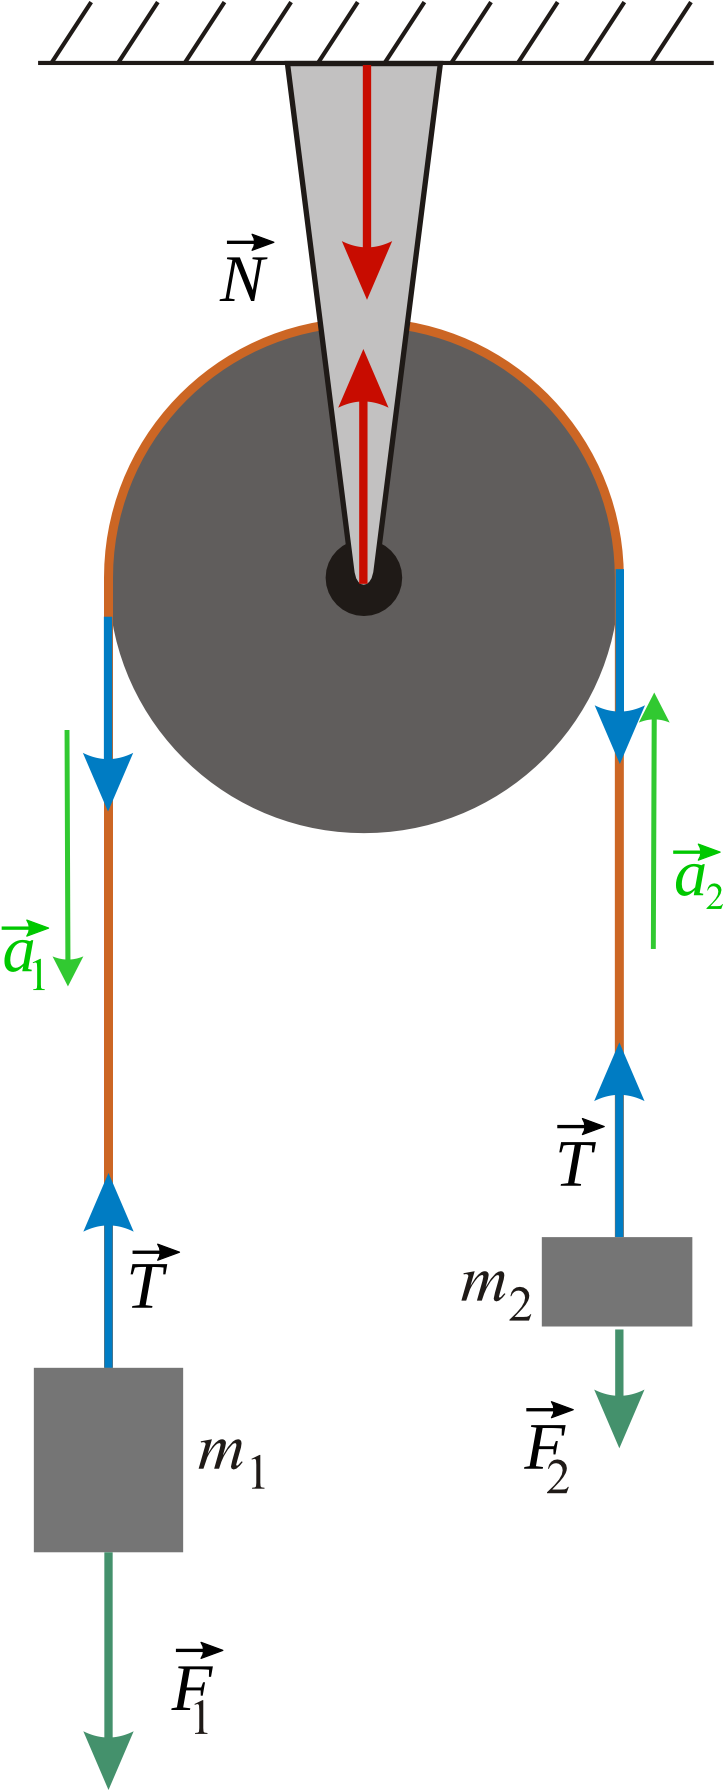
\includegraphics[width=0.5\textwidth]{immagini/atwood_1.png}
 % atwood_1.png: 723x1790 pixel, 600dpi, 3.06x7.58 cm, bb=0 0 87 215
 \caption{Attenzione le lunghezze dei vettori forza non sono in scala}
 \label{fig:atwood}
\end{figure}
\section*{Caso Statico}
Nal caso statico le masse $m_1$ ed $m_2$ sono uguali per cui la forza peso e la tensione si bilanciano perfettamente.
Per la prima massa possiamo scrivere:
\begin{equation}
 \mathbf{T}+\mathbf{F}_1=0
\end{equation}

o prescindendo dalla natura vettoriale dato che il problema si svolge in una sola dimensione:
\begin{equation}
 T-F_1=0
\end{equation}
con $F_1=m_1g$
ripetendo lo stesso ragionamento per la seconda massa otteniamo:
\begin{equation}
 T-F_2=0
\end{equation}
con $F_2=m_2g$. La reazione vincolare della carrucola sul soffitto sarà, come si vede dalla figura [\ref{fig:atwood}]:
\begin{equation}
 N=2T
\end{equation}
poiché la carrucola esercita tramite il filo una forza in modulo pari a $T$ su ognuna delle masse sospese e per il terzo principio della dinamica anche le masse sospese esercitano la stessa forza sulla carrucola.
Quindi otteniamo:
\begin{equation}
 N=2(m_1+m_2)g=2mg
\end{equation}

\section*{Caso dinamico}
Se le masse sospese non sono identiche il sistema comincerà a muoversi nel verso della massa più grande. Immaginiamo che sia $m_1>m_2$ e che quindi in figura [\ref{fig:atwood}] la massa a sinistra cada verso il basso mentre la massa a destra salga verso l'alto. Siccome le due masse sono collegate da un filo inestensibile l'accelerazione, in modulo, dovrà essere la medesima per cui si potrà scrivere:
\begin{equation}
 \mathbf{a}_1=-a\mathbf{\hat y}
\end{equation}

e
\begin{equation}
 \mathbf{a}_2=a\mathbf{\hat y}
\end{equation}

dove $a=|\mathbf{a}_1|=|\mathbf{a}_2|$ e $\mathbf{\hat y}$ è un versore  perpendicolare al soffitto e diretto verso l'alto in figura [\ref{fig:atwood}].
In questo caso le forze totali agenti sulle masse  non saranno più nulle per cui vedremo gli oggetti sospesi muoversi. Per calcolare il modulo dell'accelerazione ripetiamo quanto fatto nel caso statico, trattando il problema unidimensionalmente:
\begin{equation}
 T-F_1=T-m_1g=-am_1
\end{equation}
e
\begin{equation}
 T-F_2=T-m_2g=am_2
\end{equation}

possiamo così scrivere il sistema
\begin{equation}
\begin{cases}
 T-m_1g=-am_1\\
 T-m_2g=am_2
\end{cases}
\end{equation}

risolvendo tale sistema otteniamo i dati richiesti
\begin{equation}
 \begin{cases}
  a=g\dfrac{m_1-m_2}{m_2+m_1}\\
\\
  T=g\dfrac{m_1m_2}{m_1+m_2}
 \end{cases}
\end{equation}
quanto abbiamo detto nel caso statico circa la reazione vincolare del soffitto rimane valido anche nel caso dinamico cosa che ci permette di concludere che:
\begin{equation}
 N=2T=2g\dfrac{m_1m_2}{m_1+m_2}
\end{equation}



\end{document}
